\chapter{Results - Example Analysis - the `top` process}
\label{cha:results}

For the example analysis using the produced program, the \verb|top v4.0.4| \cite{warner_procps-ng_2023} program was used on the development machine.
This program is a utility that provides a terminal utility for displaying active processes and their usage.
The development machine is running a WSL virtualized Linux distribution on Intel's 11th generation i5-1145G7 4 core processor. 
The Linux distribution used is \verb|NixOS 25.05.20241229.88195a9 (Warbler) x86_6| running \verb|Linux 5.15.167.4-microsoft-standard-WSL2| kernel version.
The first step in analysis reproduction is to launch the \verb|top| program on the command line and push the process into the background with the \verb|&| operator.
Afterwards the binary was called (used cargo's run command to compile the program from scratch with the release mode flag). The command line option provided to the binary (after -- ) is the process id and error as the minimum log level to avoid unnecessary verbosity (see \autoref{fig:cli-run}).

\begin{figure}
    \centering
    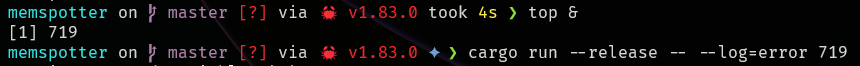
\includegraphics[width=1\linewidth]{cli-run.png}
    \caption{Invoking the program in the shell after launching a background process}
    \label{fig:cli-run}
\end{figure}

\section{Brief UI overview}

After launching the program, the initial state of the code section shows the disassembled executable segment of the \verb|top| binary.
The header shows the information about the running process id, while the picker section shows all the linked libraries and highlights the actively selected one \autoref{fig:tui-main}.

\begin{figure}
    \centering
    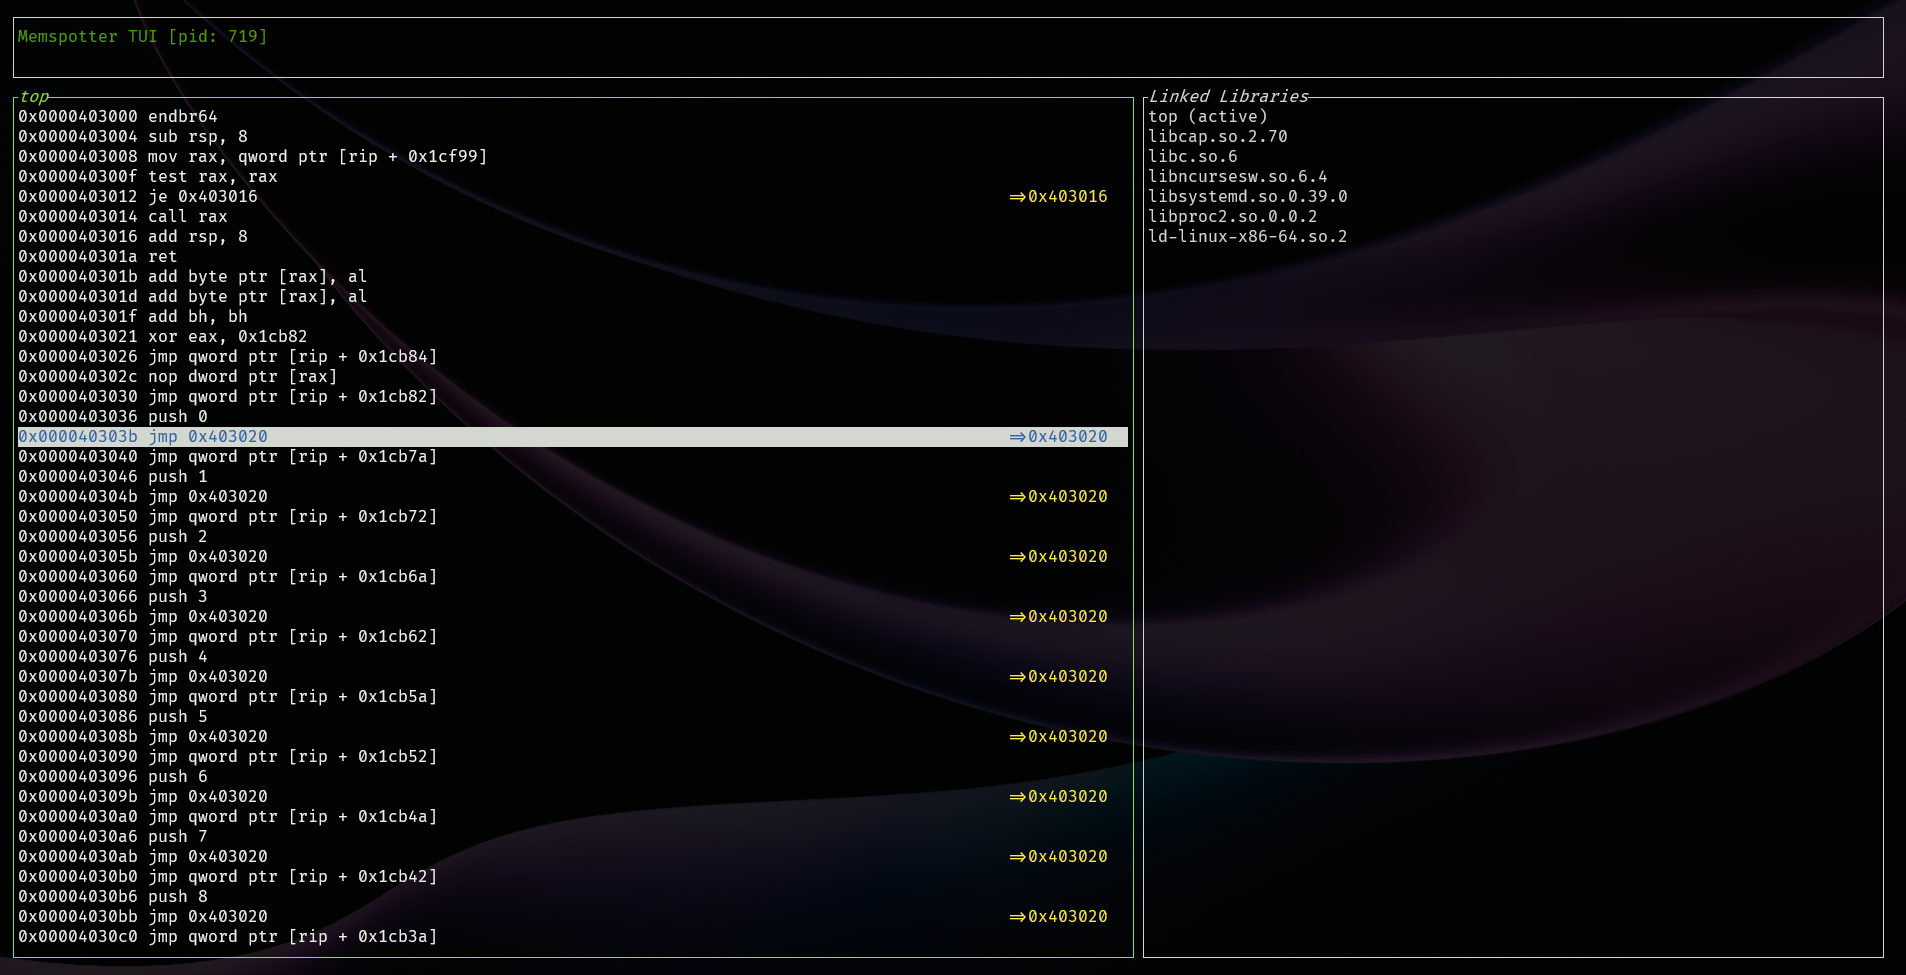
\includegraphics[width=1\linewidth]{tui-main.png}
    \caption{The main user interface after launching the program}
    \label{fig:tui-main}
\end{figure}

\section{Main function and its calls}

By changing to the function view of the library (right arrow, and then tab), the functions of the executable become visible.
Then, using the arrow keys, the main function can be found and navigated with the enter key.
Afterwards the code section makes the main function fragment focused beginning from the function start.
From there the code of the function can be seen as well as the functions being called on the jump and call instructions such as \verb|atexit| or \verb|initialize_nls| (see \autoref{fig:function-picker}).
The user can then use the picker pane to navigate to the chosen function to deepen the analysis and follow the possible code paths.

\begin{figure}
    \centering
    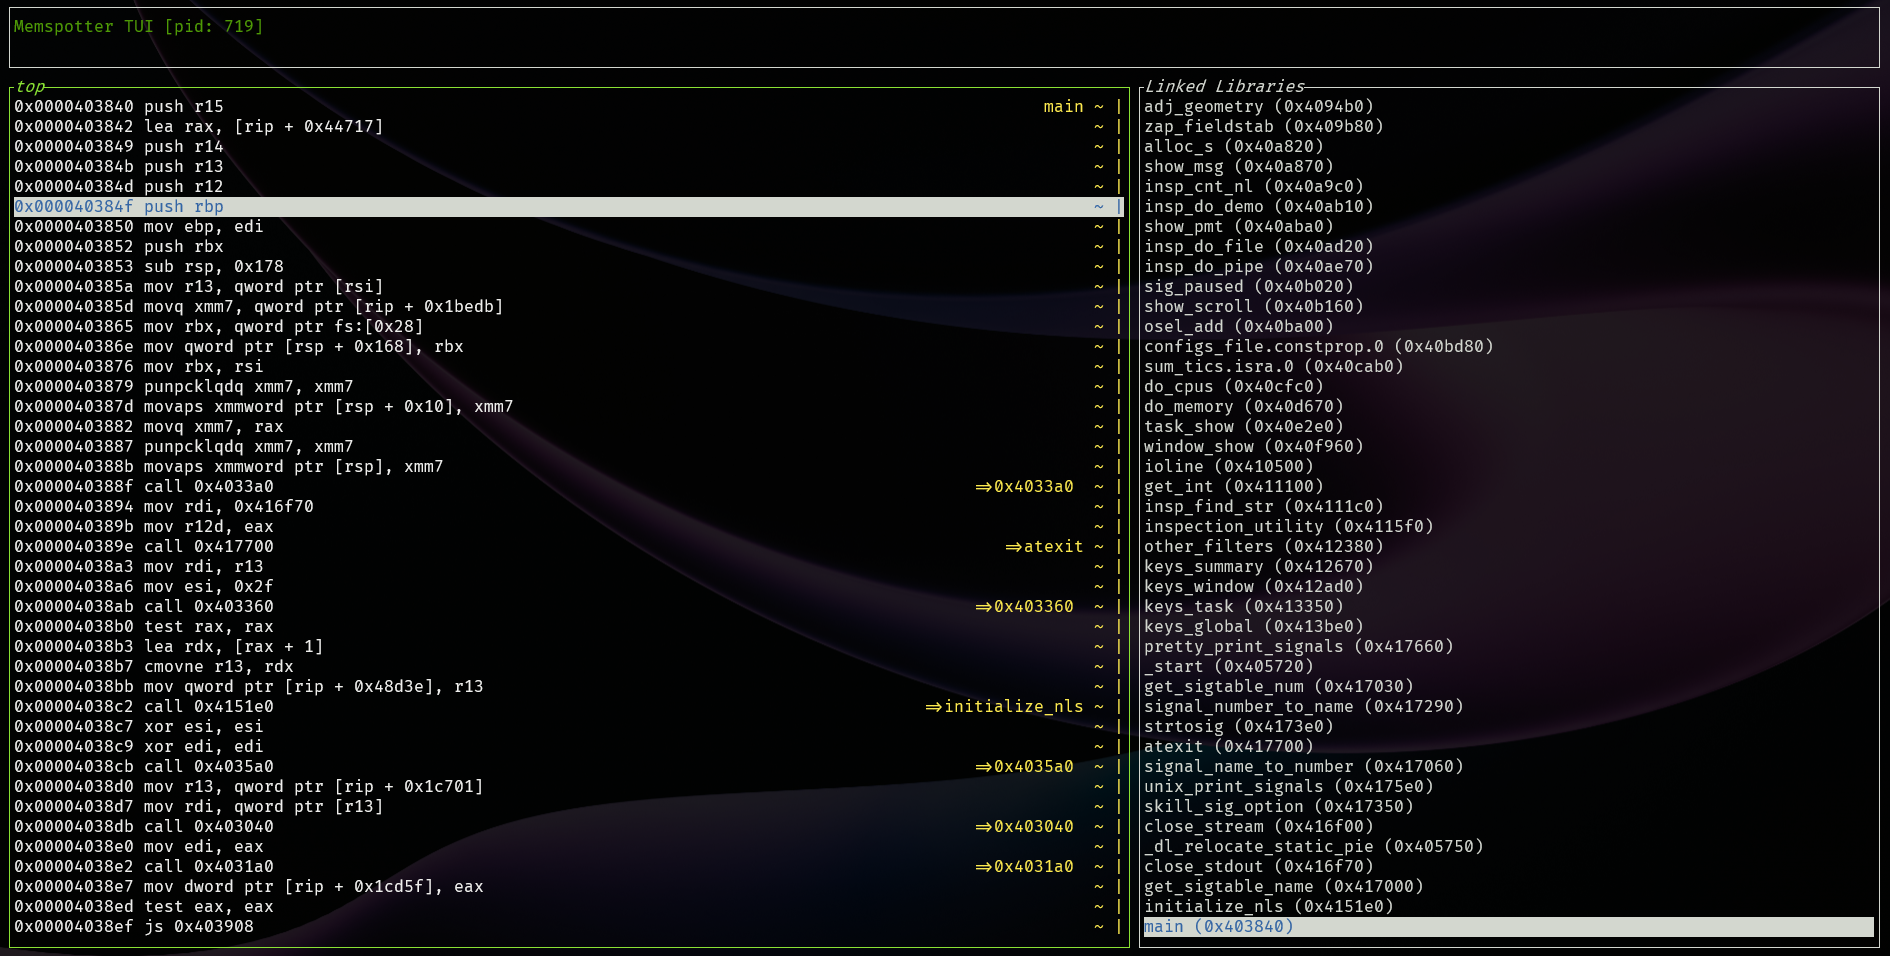
\includegraphics[width=1\linewidth]{tui-function-select.png}
    \caption{Main executable function with function selection menu opened}
    \label{fig:function-picker}
\end{figure}

\section{Brief look at dependencies}

Taking a look at the dependency picker in \autoref{fig:function-picker} , in addition to the main executable, the program links to 6 other dynamic libraries.
The most obvious and possibly important ones are first the C standard library (\verb|libc.so.6|) and the GNU dynamic linker (\verb|ld-linux.so.2|).
Even by briefly looking at the picker section an educated user can ascertain the major versions of the linked libraries by the file extensions - in this case the linker uses major version 2 and the C standard library has major version 6. 
Furthermore, the user can select any of the shared libraries to set them as active and view their executable sections in the left pane.
Additionally, all of the linked libraries can be swapped to function view by using the tab key to allow fast scrolling to specific library functions in the disassembled view.

\begin{figure}
    \centering
    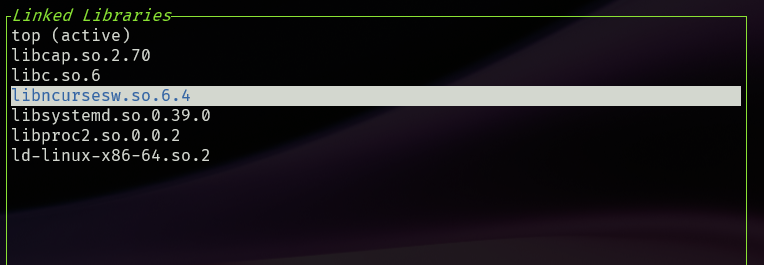
\includegraphics[width=0.7\linewidth]{tui-lib-select.png}
    \caption{Library selection window}
    \label{fig:lib-select}
\end{figure}

\section{Notable discoveries}

\subsection{cold and hot function markers}

Digging deeper into the assembly code of the libraries, some link-time optimizations can be spotted.
The main one is the annotations of the \verb|.cold| function and how the dynamic linker reacts to them.
Cold is one of the parameters that can annotate the shared library and is responsible for marking the function as possibly unused \cite{noauthor_common_nodate}.
The behavior for the Linux dynamic linker in such situations is to group these functions together, closer to the end of the allocated memory space to make way for the more used functions.
This can also possibly improve the cache locality and prediction rate due to designating a specific region for the unused functions rather than placing them in regular places where they may take cache space from more used functions. 
An example of such cold space can be seen in \autoref{fig:cold-func} where a cold function is highlighted in the right sections, and two cold function start symbols can be seen in the code section (\verb|__assert_fail_base.cold| and \verb|_nl_load_domain.cold|)

\begin{figure}
    \centering
    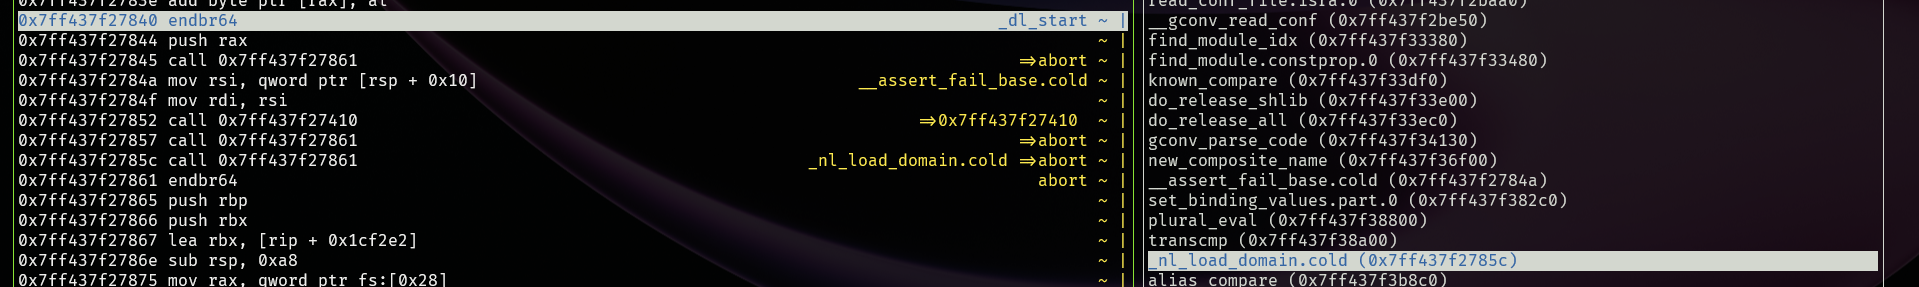
\includegraphics[width=1\linewidth]{cold-starts.png}
    \caption{Code fragment highlighting function marked as cold}
    \label{fig:cold-func}
\end{figure}

\subsection{pratitioning and inlining}

Another optimization that can be looked at is the use of different function-like symbols to the symbol table, the most notable of which are function part markers.
The cause of \verb|.part| annotations in the assembly instructions is due to the IPA optimizations of the GCC compiler \cite{noauthor_ipa_nodate}.
In such cases the compiler can deem it more optimal to inline some parts of the functions into general code and invoke the rest only on specific condition (e.g. in the case of a function usually returning early).
Furthermore, those optimizations can also be applied to loops with conditionals or breaks, switch statements, or even to inline whole functions if they are called a sufficiently small number of times.
During the analysis, these optimizations can most likely be found within the most performance-critical libraries, for example, in system libraries such as the c standard library (see \autoref{fig:function-parts}).

\begin{figure}
    \centering
    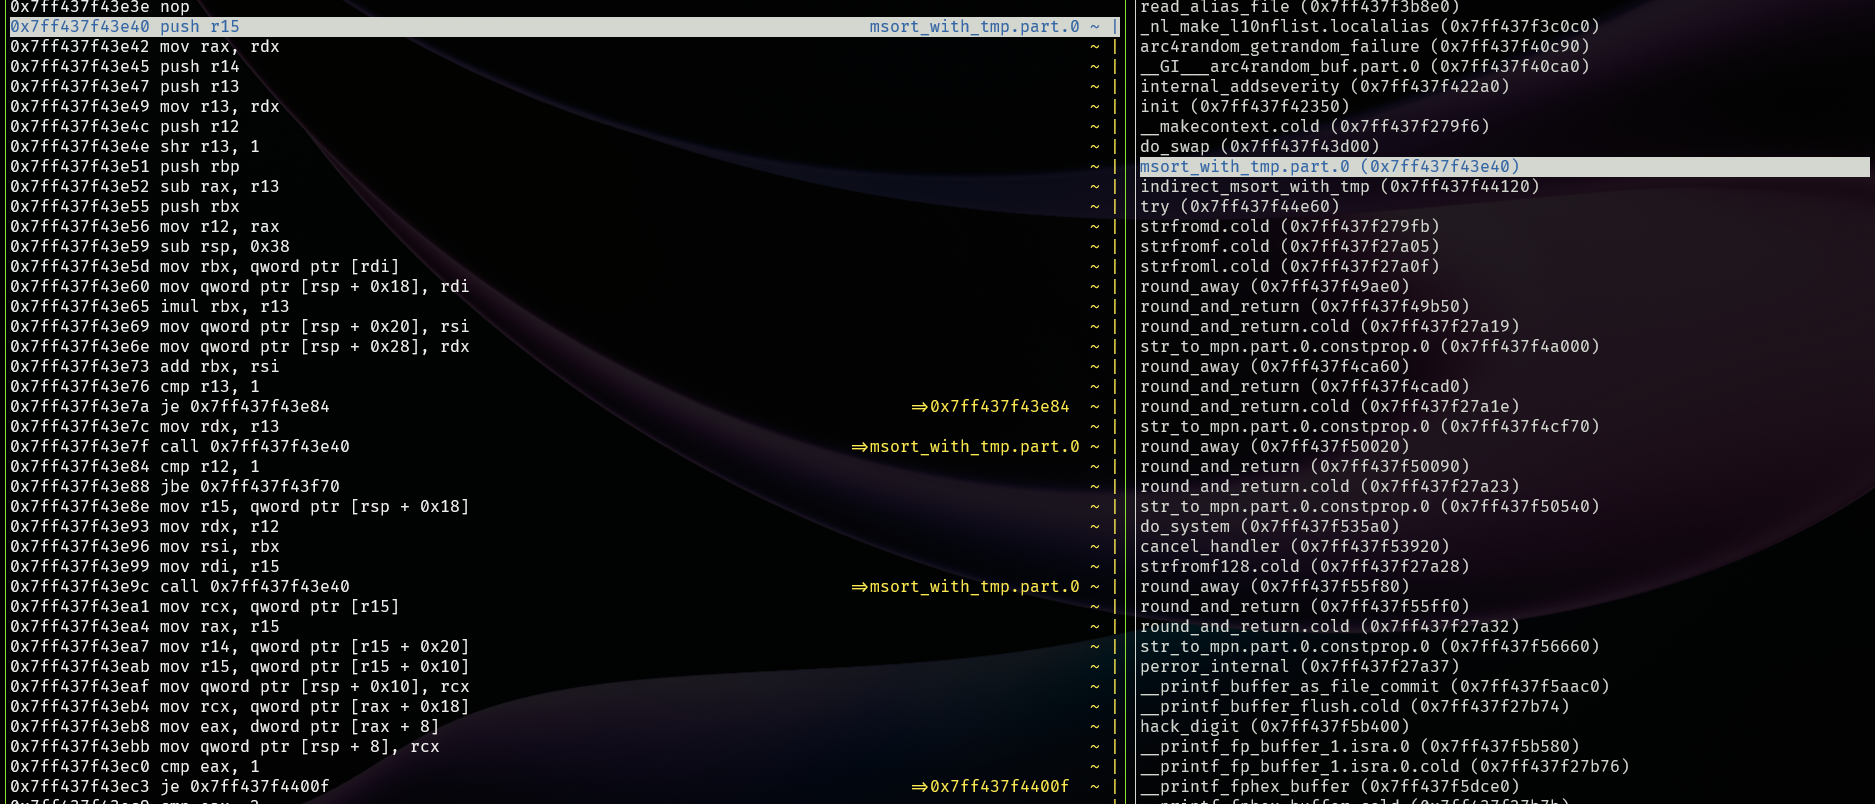
\includegraphics[width=1\linewidth]{function-parts.png}
    \caption{Assembly code fragment with a function part symbol highlighted}
    \label{fig:function-parts}
\end{figure}

\subsection{SIMD specific instructions}

The last of the optimizations that can be seen in the analysis is the usage of vector instructions.
This is also an optimization generated by the GCC compiler, when provided with information about the specific microcode architecture \cite{noauthor_x86_nodate}, or by explicitly invoking the functions in the code.
As the NixOS operating system like Gentoo Linux distribution compiles most of its libraries on the machine, it is able to pass such capability information to the compiler.

In this case, Intel-specific SIMD instructions are available such as \verb|movaps| which sets the address of SIMD-packed instructions and \verb|punpcklqdq| which is one of the unpacked SIMD instructions \cite{intel_corporation_intel_2024} (see \autoref{fig:simd-instructions}).

\begin{figure}
    \centering
    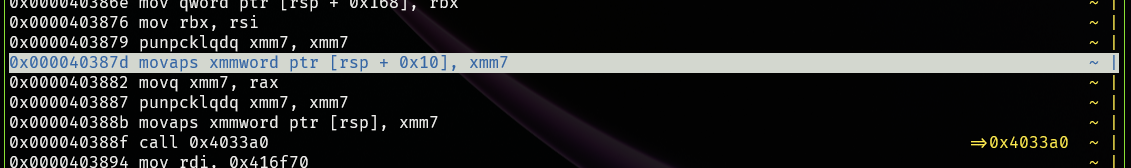
\includegraphics[width=1\linewidth]{arch-specific-instruction.png}
    \caption{Assembly code fragment showing Intel-specific SIMD instructions}
    \label{fig:simd-instructions}
\end{figure}

\subsection{Analysis applications}
All of the information collected from this inspection can also be used in a reverse engineering concept.
Searching for such characteristics while analyzing an unknown library or code fragment, optimizations, and SIMD-specific instructions can provide information about the chip manufacturer and specific microcode architecture and compiler options.
Furthermore, compiler linking specific versions of libraries can help infer information about the time at which software was developed, and functions marked as cold or hot can tell information about usage patterns of specific functions within those libraries.